\documentclass[journal]{IEEEtran}
\usepackage[utf8]{inputenc}
\usepackage[T1]{fontenc}
\usepackage{amsmath,amssymb}
\usepackage{graphicx}
\usepackage{booktabs}
\usepackage{array}
\usepackage{url}
\usepackage{cite}
\usepackage{xcolor}
\usepackage{balance}
\usepackage[hidelinks]{hyperref}

\graphicspath{{../outputs/figures/}}
\newcommand{\nSeeds}{5}
\newcommand{\nEpochs}{20}
\newcommand{\hiddenDim}{64}
\newcommand{\textDim}{128}
\newcommand{\subsetPct}{100}
\newcommand{\nBoot}{1000}
\newcommand{\lr}{0.003}
\newcommand{\batchSize}{256}
\newcommand{\maxHistory}{50}
\newcommand{\maxContext}{6}
\newcommand{\cfTau}{0.1}
\newcommand{\cfDom}{1.5}
\newcommand{\persistK}{2}
\newcommand{\minHist}{3}
\newcommand{\injRate}{0.15}
\newcommand{\nTestNat}{4472}
\newcommand{\nTestSyn}{624}
\newcommand{\nTrain}{36883}
\newcommand{\torchVersion}{2.14.0+cpu}
\newcommand{\pythonVersion}{3.12.8}
\newcommand{\cpuCount}{8}
\newcommand{\lambdaRel}{1.0}
\newcommand{\lambdaAct}{0.6}
\newcommand{\conflictLossWeight}{2.0}
\newcommand{\relLabelSmoothing}{0.1}
\newcommand{\selfTrainStart}{3}
\newcommand{\selfTrainMinConf}{0.6}
\newcommand{\selfTrainThreshold}{0.9}
\newcommand{\nConflictStrict}{331}
\newcommand{\nConflictBroad}{1272}
\newcommand{\nConflictSyn}{226}
\newcommand{\disagreementConfMin}{0.6}
\newcommand{\disagreementJsMin}{0.5}


\begin{document}

\title{Adaptive Intent--Preference Arbitration for Conversational Recommendation: A Reproducible Study on ReDial}

\author{Dhaya~R%
\thanks{D.~R is with [affiliation]. E-mail: dhayanidhi.r@gmail.com.}%
\thanks{Code, configuration, generated figures and the executed notebook are available at \url{https://github.com/dhayarajas/AIPA-CRS}.}}

\markboth{Manuscript draft}{R: Adaptive Intent--Preference Arbitration for Conversational Recommendation}

\maketitle

\begin{abstract}
A conversational recommender hears two voices at once: what a user has liked over many sessions, and what they are asking for in the current conversation. Most systems blend the two with a fixed rule and hope for the best. That works when the signals agree and fails quietly when they do not, for example when a habitual comedy viewer asks for a war film for the weekend. We study \emph{Adaptive Intent--Preference Arbitration} (AIPA), a model that first classifies the relationship between the long-term preference (LTP) and the short-term intent (STI) into one of five categories (complement, consistent, conflict, override, uncertain), then chooses an action (fuse, prioritise LTP, prioritise STI, or ask a clarifying question), and finally re-ranks candidates with weights that depend on that decision. Two further components track whether an intent shift repeats across sessions and should be absorbed into the long-term profile, and probe the trained model with counterfactual ablations of each signal to report which one actually drove a recommendation. We build the whole pipeline on ReDial, an English human--human movie recommendation corpus, deriving cross-session profiles from recurring seeker identities and using MovieLens genres as item metadata. Because ReDial has no relationship annotations, labels come from a transparent weak-rule scheme and from controlled synthetic conflict injection, and every result is reported separately for the two sources. In the reduced-budget run reported here (\subsetPct\% of the data, \nSeeds{} seeds) AIPA is clearly better than a profile-only recommender and than a GRU sequential baseline, but it does not separate from an intent-only model or from simple adaptive fusion, and the ablations are statistically flat. The arbitration head itself behaves sensibly: clarification precision is above 0.97 and wrong overrides are rare. We report these outcomes as they are, discuss why the central hypothesis is not yet supported, and list the concrete steps needed for a conclusive test. All numbers, tables and figures in this paper are generated by the released code.
\end{abstract}

\begin{IEEEkeywords}
Conversational recommender systems, user intent, long-term preference, preference conflict, clarification, counterfactual analysis, reproducibility.
\end{IEEEkeywords}

\IEEEpeerreviewmaketitle

\section{Introduction}
\IEEEPARstart{R}{ecommender} systems that talk to their users have an advantage that click-based systems lack: the user can simply say what they want right now. The flip side is that this fresh signal has to be reconciled with everything the system already knows about the person. Someone who has spent years watching dramas may ask, on a Friday night, for ``something dumb and funny''. A system that follows its profile ignores the request; a system that follows the request may throw away a decade of evidence for a single evening. Neither extreme is right, and the right answer depends on the situation.

The bulk of work on conversational recommendation (CRS) has focused on how to elicit preferences within a dialogue \cite{christakopoulou2016towards,sun2018crm,lei2020ear,zhang2018conversational} or how to ground dialogue in knowledge about items \cite{chen2019kbrd,zhou2020kgsf}. How to reconcile what is said now with what was learned before has received much less direct attention. When both signals are used, they are usually combined with a fixed rule or a learned gate that is never asked to explain itself, and evaluation almost never singles out the turns where the two disagree. Yet those are exactly the turns where the design choice matters.

This paper treats the reconciliation step as a first-class problem. We call it \emph{arbitration}, and we make it explicit in three ways. First, the model predicts what kind of relationship holds between the long-term preference (LTP) and the short-term intent (STI): they may reinforce each other, one may add a new dimension the other lacks, they may contradict each other, the user may explicitly set the profile aside, or there may simply be too little evidence to tell. Second, this relationship drives a discrete action (fuse the signals, favour one of them, or ask a question) and the action in turn sets the fusion weights. Third, the model is made to account for its recommendations: after training we knock out one signal at a time and measure how much the ranking moves, giving a per-turn label of which signal drove the recommendation. We stress that this is a diagnostic of the fitted model, not a causal claim about users.

Our second aim is a clean and fully reproducible experimental base. We deliberately use ReDial \cite{li2018redial}, an English corpus of human--human movie dialogues. It has no cross-session profiles by design, but crowd workers recur across many dialogues, and we use that recurrence to construct chronological seeker histories under strict no-look-ahead rules. ReDial also has no labels for our relationship taxonomy; rather than pretend otherwise, we derive weak-rule labels from the dialogue text and additionally inject controlled synthetic conflicts, and we never mix the two in a table. Every claim about a metric is accompanied by bootstrap intervals and paired tests with multiple-comparison correction.

The results of the run reported here are mixed, and we say so. AIPA improves on profile-only and sequential baselines by a clear margin, its arbitration behaviour is sensible, and the counterfactual probe agrees with the chosen action on a majority of controlled cases. It does not, however, outperform an intent-only recommender or plain adaptive fusion, and none of the ablations reach significance. We see the contribution of this paper as the framing, the evaluation protocol, and an honest baseline measurement that later work can build on; the discussion in Section~\ref{sec:discussion} lists what a decisive test would need.

\section{Related Work}
\subsection{Conversational recommendation}
Early CRS work framed the dialogue as a preference elicitation game in which the system asks about attributes and the user answers \cite{christakopoulou2016towards,sun2018crm}. Estimation--Action--Reflection \cite{lei2020ear} formalised the choice between asking and recommending as a policy problem. The ``system ask, user respond'' paradigm of Zhang \emph{et al.}\ \cite{zhang2018conversational} likewise treats clarifying questions as an action to be planned. Our clarification action sits in this tradition but is triggered by the relationship between two evidence sources rather than by attribute uncertainty alone.

Open-ended, natural-language CRS became tractable with ReDial \cite{li2018redial}, followed by knowledge-grounded models such as KBRD \cite{chen2019kbrd} and KGSF \cite{zhou2020kgsf}, and by further corpora including INSPIRED \cite{hayati2020inspired} and the Chinese TG-ReDial \cite{zhou2020tgredial}. TG-ReDial is the only one of these that ships per-user histories, but its dialogues are in Chinese; we chose ReDial so that data, labels, case studies and error analysis could all be read in English, and reconstructed histories from recurring seekers instead. Surveys by Jannach \emph{et al.}\ \cite{jannach2021survey} and Gao \emph{et al.}\ \cite{gao2021advances} give a broader map of the field; both note that reconciling the conversation with the historical profile remains open.

\subsection{Long- and short-term signals}
Session-based and sequence-aware recommenders \cite{hidasi2016gru4rec,kang2018sasrec,quadrana2018sequence} learn to weigh recent behaviour against older behaviour implicitly, through the recurrence or the attention pattern. Our sequential baseline follows this recipe. The difference in AIPA is that the weighing is exposed: the relationship class and the action are discrete, supervised (weakly) and inspectable, and the fusion weights are a function of them.

\subsection{Counterfactual reasoning in recommendation}
We borrow the vocabulary of interventions \cite{pearl2009causality} for the driver diagnostic, but the object we intervene on is the trained model, not the user. Zeroing the LTP encoding and re-scoring tells us how much the model's output depends on that pathway, which is a form of ablation-based attribution. We do not claim identification of any causal effect on user behaviour, and we avoid the word ``effect'' when describing these numbers.

\section{Problem Formulation}
\label{sec:problem}
Consider a seeker $u$ with a chronologically ordered set of past dialogues $\mathcal{H}_u = \{D_1, \dots, D_{m}\}$ and a current dialogue $D_{m+1}$. At turn $t$ of $D_{m+1}$ the recommender introduces a new movie $y_t$. Our prediction target is $y_t$, and the evidence available is:
\begin{itemize}
  \item \textbf{Long-term preference (LTP)}: the movies $u$ marked as liked or seen in $D_1,\dots,D_m$, the genre distribution over those movies, and short self-descriptive sentences (``I usually go for thrillers'') extracted from earlier dialogues;
  \item \textbf{Short-term intent (STI)}: the seeker's utterances in $D_{m+1}$ strictly before turn $t$, the movies mentioned so far in the dialogue, a genre distribution induced from those utterances and mentions, and lexical flags (negation, explicit override markers such as ``for a change'', explicit habit markers such as ``as usual'').
\end{itemize}
Nothing from turn $t$ onward, and nothing from later dialogues, is visible to the model.

We define five \textbf{relationship} classes between LTP and STI. \emph{Consistent}: STI points where LTP already points. \emph{Complement}: STI adds a dimension that LTP does not cover but does not contradict it. \emph{Conflict}: STI opposes LTP with no signal that the user is aware of it. \emph{Override}: STI opposes LTP and the user explicitly flags a deliberate departure. \emph{Uncertain}: too little evidence on either side. The \textbf{action} space is $\{$Fuse, Prioritise\_LTP, Prioritise\_STI, Ask\_Clarification$\}$. A relationship implies a default action (consistent$\to$fuse, complement$\to$fuse, conflict$\to$prioritise STI, override$\to$prioritise STI, uncertain$\to$ask), but the learned policy is free to depart from it.

We further distinguish a \textbf{temporary override}, which affects only the current session, from a \textbf{persistent shift}, in which the same departure recurs across $k$ or more distinct sessions and should be folded into LTP.

\section{Method}
\label{sec:method}
Figure~\ref{fig:arch} shows the components. All encoders are small because the point of the study is the arbitration logic, not representational power; the same item tower, dimensionality and training recipe are used for every baseline so that differences are attributable to the arbitration design.

\begin{figure}[t]
  \centering
  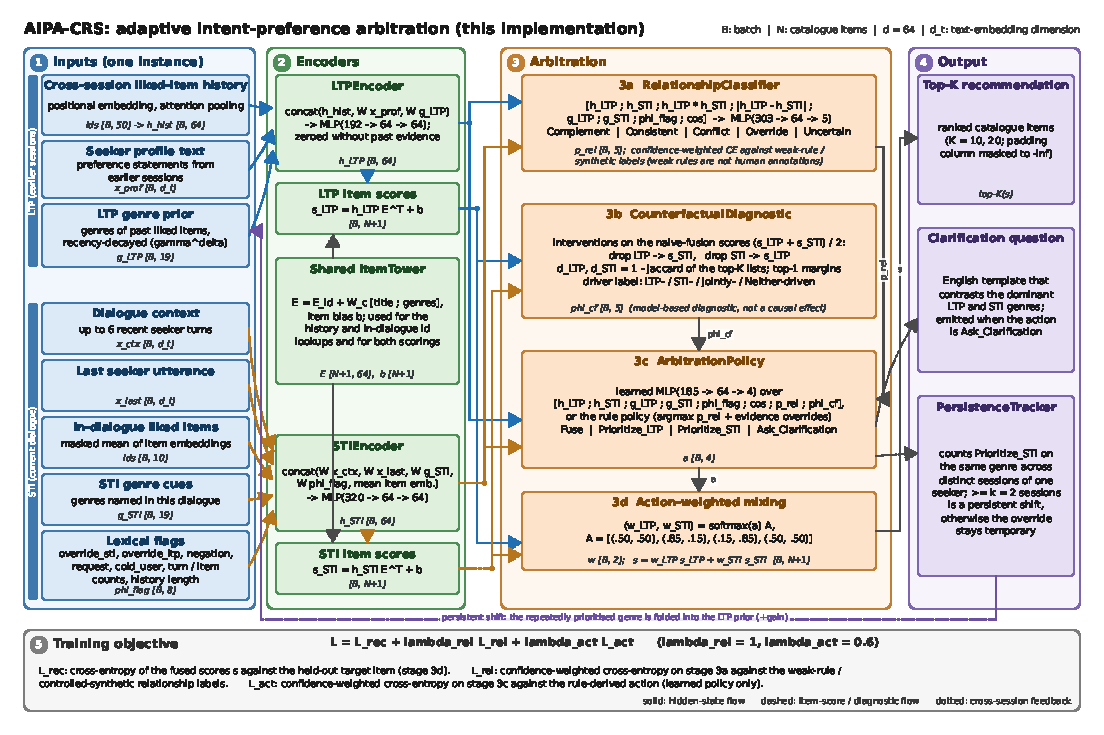
\includegraphics[width=\columnwidth]{fig00_architecture}
  \caption{AIPA components. History and dialogue context feed separate LTP and STI encoders. A relationship classifier and a counterfactual driver probe inform the arbitration policy, which produces fusion weights (or a clarifying question). A persistence tracker decides whether repeated intent shifts should update the long-term profile.}
  \label{fig:arch}
\end{figure}

\subsection{Item and signal encoders}
Each movie is represented by a learned embedding plus a projection of its content vector (TF--IDF over English title and genre text reduced with truncated SVD to \textDim{} dimensions, concatenated with a genre indicator from MovieLens \cite{harper2015movielens}). The \textbf{LTP encoder} pools the item embeddings of the seeker's history with exponentially decaying weights (older sessions count less), concatenates the LTP genre distribution and an encoding of profile sentences, and passes the result through a two-layer MLP. The \textbf{STI encoder} does the same with the encoded recent seeker text, the current-dialogue item mentions, the STI genre distribution and the lexical flags. Both encoders output a vector of dimension \hiddenDim.

\subsection{Relationship classifier and arbitration policy}
The relationship classifier takes $[h_{\text{LTP}}; h_{\text{STI}}; h_{\text{LTP}}\odot h_{\text{STI}}; |h_{\text{LTP}}-h_{\text{STI}}|]$ together with hand-crafted comparison features (cosine similarity of genre distributions, top-genre agreement, history length, cold-start flag, lexical flags) and outputs a distribution over the five relationships. The arbitration policy consumes the relationship distribution, the same comparison features and the counterfactual features described below, and outputs a distribution over the four actions. Fusion weights are computed as
\begin{equation}
  w_{\text{LTP}} = \sum_a p(a)\, \beta_a, \qquad w_{\text{STI}} = 1 - w_{\text{LTP}},
\end{equation}
where $\beta_a$ is a learned scalar per action initialised at $0.5$ for Fuse and Ask, $0.8$ for Prioritise\_LTP and $0.2$ for Prioritise\_STI. The final score is $s(i) = e_i^\top(w_{\text{LTP}} h_{\text{LTP}} + w_{\text{STI}} h_{\text{STI}}) + b_i$. A \emph{rule policy} variant replaces the learned action head by the default relationship$\to$action table; it is used as an ablation.

\subsection{Clarification}
When the chosen action is Ask\_Clarification and the model's confidence in that action exceeds a threshold, the system emits an English question generated from a small template set that names the top LTP genre and the top STI cue, for example \emph{``You usually go for dramas but you mentioned horror just now---should I stick with dramas tonight or try horror?''} Offline we cannot observe the user's answer, so we evaluate clarification by its precision (was the reference label indeed uncertain or conflicting?) and by an efficiency proxy (would the target have been reachable from the top-20 without asking?).

\subsection{Counterfactual driver diagnostic}
After training, for each test turn we re-score the candidates three times: normally, with $h_{\text{LTP}}$ zeroed, and with $h_{\text{STI}}$ zeroed. Let $\delta_{\text{LTP}}$ and $\delta_{\text{STI}}$ be the fractions of the original top-$K$ list that change when the respective signal is removed. The turn is labelled \emph{Neither-driven} if both are below $\tau=\cfTau$; \emph{STI-driven} if $\delta_{\text{STI}}\ge\tau$ and $\delta_{\text{STI}}\ge\cfDom\,\delta_{\text{LTP}}$; \emph{LTP-driven} symmetrically; and \emph{Jointly-driven} otherwise. The two $\delta$ values also enter the policy as features, so the model can learn to prefer clarification when both signals are pulling the list in different directions. Again, these are statements about the model's sensitivity, not about the user.

\subsection{Temporary versus persistent shifts}
The persistence tracker records, per seeker, the genre that won arbitration whenever the predicted action was Prioritise\_STI. If the same genre wins in at least $k=\persistK$ distinct sessions, later instances of that seeker receive an LTP genre vector shifted toward it, and the event is logged. Shifts that do not recur remain session-local. In the offline setting this is evaluated by counting detected shifts and by checking that the full model and the model with the tracker disabled differ only on affected seekers.

\subsection{Training}
The recommendation loss is a sampled softmax over the item catalogue. When labels are available, a cross-entropy term on the relationship head (weight $\lambda_{\text{rel}}=0.5$) and one on the action head ($\lambda_{\text{act}}=0.3$) are added, each weighted per instance by the label confidence so that low-confidence weak labels contribute less. We train with AdamW \cite{loshchilov2019adamw}, learning rate \lr, batch size \batchSize, gradient clipping at 1.0, and early stopping on validation Hit@10 with a patience of three epochs. For the ``without clarification'' ablation, Ask\_Clarification targets are remapped to Fuse during training as well as masked at inference, so the ablation is not merely a decoding constraint.

\section{Data and Labels}
\label{sec:data}
\subsection{ReDial and cross-session histories}
ReDial \cite{li2018redial} contains 11{,}348 English dialogues (10{,}006 training, 1{,}342 test) between a seeker and a recommender, with per-movie seeker annotations for \emph{liked}, \emph{seen} and \emph{suggested}. We split 1{,}000 training dialogues off as validation. The corpus has 764 distinct seeker identifiers and most seekers appear in many dialogues (Fig.~\ref{fig:data}). We order a seeker's dialogues by conversation identifier and treat this as chronological order; this is an assumption we could not verify against timestamps, and we flag it as such. For dialogue $D_{m+1}$, LTP is built only from $D_1,\dots,D_m$; a seeker with fewer than \minHist{} earlier sessions is treated as cold. Item metadata (genres, years) come from MovieLens \emph{ml-latest} \cite{harper2015movielens} joined on normalised title and year; movies without a match keep an empty genre vector rather than an imputed one.

\begin{figure}[t]
  \centering
  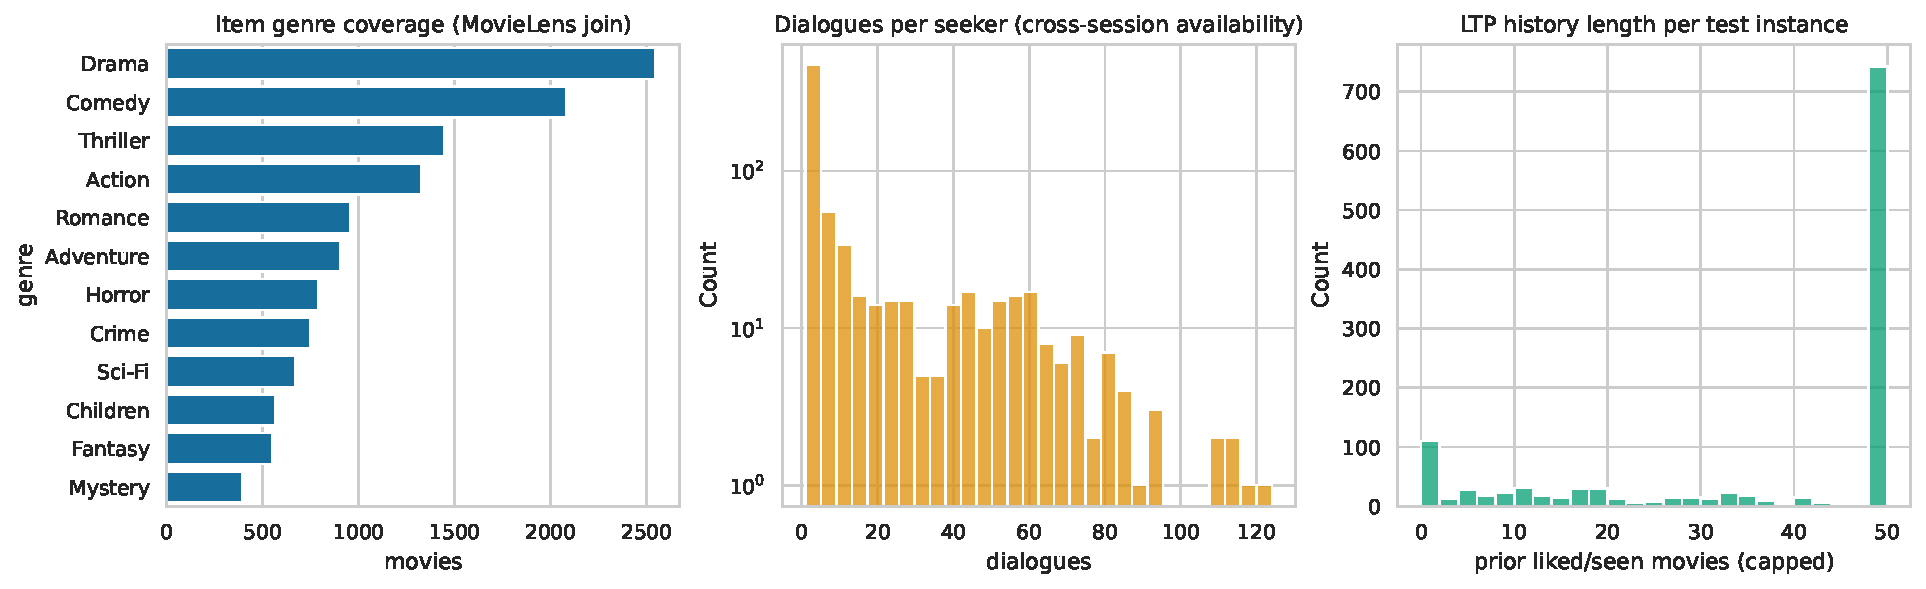
\includegraphics[width=\columnwidth]{fig01_dataset_overview}
  \caption{ReDial overview: dialogue counts per split, dialogues per seeker, genre coverage after the MovieLens join, and turns per dialogue.}
  \label{fig:data}
\end{figure}

Each recommendation instance is one (dialogue, turn, target movie) triple where the recommender introduces a movie not yet mentioned in the dialogue. Only the preceding \maxContext{} turns of context and at most \maxHistory{} history items are used. In the run reported here we sample \subsetPct\% of the dialogues in every split with a fixed seed, which yields \nTrain{} training instances and \nTestNat{} natural test instances.

\subsection{Relationship labels}
ReDial has no relationship annotations. We use two label sources and keep them apart throughout.

\textbf{Weak-rule labels.} A deterministic procedure assigns a relationship, an action and a confidence from the LTP and STI genre distributions and from lexical evidence: explicit habit markers yield \emph{Consistent}; negation of a habitual genre or a known tension pair (e.g.\ comedy vs.\ horror) with low genre similarity yields \emph{Conflict}, or \emph{Override} when an explicit departure marker is present; a new genre dimension with otherwise compatible distributions yields \emph{Complement}; absence of genre evidence yields \emph{Uncertain}. These labels are noisy, and the confidence attached to each is used to down-weight it in training and to define the ``high-confidence'' evaluation subsets.

\textbf{Synthetic controlled labels.} For \injRate{} of natural test instances whose seeker has a usable LTP, we append one English seeker utterance requesting a genre that conflicts with, overrides, or agrees with the seeker's top habitual genre, at one of three intensities (from a mild ``maybe'' to an insistent request), and replace the target by a movie of the requested genre. Each synthetic instance records its source instance, the injected utterance, the intended relationship and the intensity, and carries an explicit synthetic flag. Synthetic instances appear in the training set as well (with the same flag) so that the relationship head sees clean examples of the rarer classes.

Table~\ref{tab:labels} gives the resulting distribution. \emph{Override} is rare in natural data, which is expected: people seldom announce that they are departing from their habits. A slot for human-verified labels exists in the pipeline; no such annotations were available for this run and every table that would have used them reports ``not run''.

\begin{table}[t]
  \centering
  \caption{Relationship label counts by source and split.}
  \label{tab:labels}
  \small
  \begin{tabular}{llrr}
\toprule
Source & Relationship & Train & Test \\
\midrule
weak\_rule & Complement & 1342 & 165 \\
weak\_rule & Conflict & 820 & 48 \\
weak\_rule & Consistent & 4113 & 514 \\
weak\_rule & Override & 83 & 14 \\
weak\_rule & Uncertain & 1840 & 336 \\
synthetic\_controlled & Complement & 240 & 31 \\
synthetic\_controlled & Conflict & 216 & 33 \\
synthetic\_controlled & Consistent & 242 & 24 \\
synthetic\_controlled & Override & 199 & 24 \\
synthetic\_controlled & Uncertain & 247 & 31 \\
\bottomrule
\end{tabular}

\end{table}

\section{Experimental Setup}
\label{sec:setup}
\subsection{Compared systems}
\emph{LTP-only} and \emph{STI-only} score items from one encoder. \emph{Naive fusion} averages the two encodings with $\alpha=0.5$; \emph{Adaptive fusion} learns a scalar gate from the two encodings but has no relationship or action head. \emph{Sequential (GRU)} runs a GRU \cite{hidasi2016gru4rec} over the concatenation of history items and current-dialogue mentions. \emph{Conversation-aware} attends over the current dialogue with the history vector as query. The latter two are our own re-implementations in the same parameter budget; they are not reproductions of any published system and should not be read as such. The AIPA ablations remove the relationship head, the counterfactual features, clarification, or the persistence tracker, or swap the learned policy for the rule table.

\subsection{Metrics and statistics}
Ranking quality is measured by Hit@$K$ (equal to Recall@$K$ with one target per instance), NDCG@$K$ and MRR@$K$ at $K\in\{10,20\}$ over the full catalogue. Relationship classification is reported as accuracy, macro-F1, weighted-F1 and per-class F1; arbitration by action accuracy against the weak-rule action, conflict-resolution accuracy, override success (target in top-10 when STI is prioritised on a conflict), clarification precision, unnecessary-clarification rate and wrong-override rate. Calibration of the relationship head is measured by expected calibration error and Brier score \cite{guo2017calibration}. Every metric is averaged over \nSeeds{} seeds; 95\% intervals are percentile bootstraps with \nBoot{} resamples over test instances; pairwise comparisons use paired $t$ and Wilcoxon tests with Holm correction \cite{holm1979simple} within each family, and we report Cohen's $d$ and Cliff's $\delta$ \cite{cliff1993dominance}. All natural-data and synthetic-data results are reported separately.

\subsection{Compute}
Everything runs on CPU (\cpuCount{} cores; PyTorch \torchVersion, Python \pythonVersion). The configuration used here (``quick'' mode) trains for at most \nEpochs{} epochs with hidden size \hiddenDim; the released configuration also defines a ``full'' mode with the complete corpus, more seeds and more bootstrap resamples, which we have not run and for which we make no claims.

\section{Results}
\label{sec:results}
\subsection{Overall ranking quality}
Table~\ref{tab:overall} and Fig.~\ref{fig:overall} report the natural test set. Two things stand out. First, the intent signal dominates on ReDial: STI-only nearly doubles LTP-only, and every model that uses STI lands between 0.085 and 0.101 Hit@10. Second, AIPA (full) sits in the middle of that band. It is significantly better than LTP-only ($\Delta=+0.037$, Holm-corrected $p<0.001$, $d=0.18$) and than the GRU baseline on the $t$-test, but its differences from STI-only, naive fusion, adaptive fusion and the conversation-aware baseline are all within noise (Table~\ref{tab:sig}).

\begin{table}[t]
  \centering
  \caption{Natural test set ($n=\nTestNat$, mean over \nSeeds{} seeds; brackets are 95\% bootstrap intervals). Rows above the rule are baselines.}
  \label{tab:overall}
  \scriptsize
  \resizebox{\columnwidth}{!}{\begin{tabular}{lccccc}
\toprule
Model & Hit@10 [95\% CI] & NDCG@10 & MRR@10 & Hit@20 & NDCG@20 \\
\midrule
LTP-only & 0.057 [0.049, 0.067] & 0.031 & 0.023 & 0.078 & 0.036 \\
STI-only & 0.110 [0.097, 0.124] & 0.057 & 0.041 & 0.156 & 0.068 \\
Naive fusion & 0.093 [0.081, 0.105] & 0.050 & 0.037 & 0.139 & 0.062 \\
Adaptive fusion & 0.083 [0.072, 0.094] & 0.047 & 0.036 & 0.130 & 0.059 \\
Sequential (GRU) & 0.063 [0.052, 0.072] & 0.034 & 0.025 & 0.102 & 0.043 \\
Conversation-aware & 0.082 [0.071, 0.093] & 0.046 & 0.035 & 0.120 & 0.055 \\
SASRec & 0.057 [0.048, 0.065] & 0.031 & 0.023 & 0.088 & 0.039 \\
KBRD-style & 0.099 [0.086, 0.109] & 0.052 & 0.037 & 0.153 & 0.065 \\
\midrule
AIPA w/o relationship & 0.090 [0.078, 0.103] & 0.047 & 0.034 & 0.139 & 0.059 \\
AIPA w/o counterfactual & 0.089 [0.075, 0.102] & 0.047 & 0.034 & 0.141 & 0.060 \\
AIPA w/o clarification & 0.098 [0.086, 0.110] & 0.055 & 0.042 & 0.147 & 0.067 \\
AIPA w/o persistence & 0.095 [0.082, 0.107] & 0.053 & 0.040 & 0.143 & 0.065 \\
AIPA (rule policy) & 0.096 [0.085, 0.108] & 0.052 & 0.038 & 0.142 & 0.063 \\
\textbf{AIPA (full)} & \textbf{0.095 [0.083, 0.107]} & \textbf{0.053} & \textbf{0.040} & \textbf{0.144} & \textbf{0.065} \\
\bottomrule
\end{tabular}
}
\end{table}

\begin{figure}[t]
  \centering
  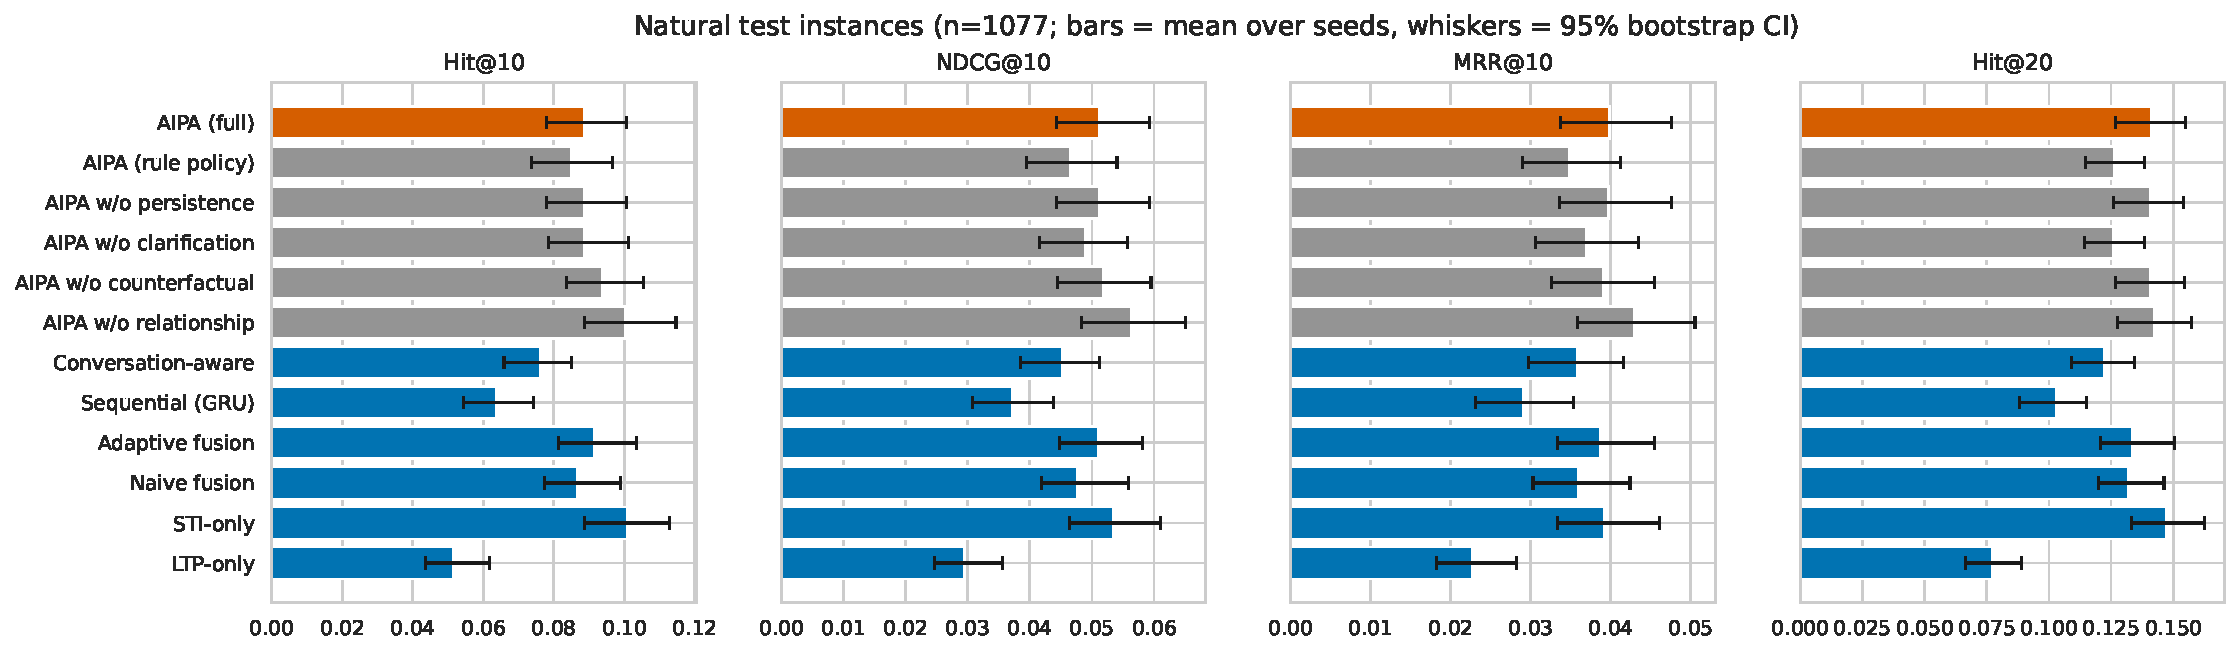
\includegraphics[width=\columnwidth]{fig03_overall_natural}
  \caption{Hit@10 and NDCG@10 on the natural test set with bootstrap intervals.}
  \label{fig:overall}
\end{figure}

\begin{table*}[t]
  \centering
  \caption{Paired comparisons of AIPA (full) against each other system on Hit@10. $\Delta$ is the mean per-instance difference (positive favours AIPA), $p_{\text{Holm}}$ the Holm-corrected paired $t$-test $p$-value ($^{*}$: $<0.05$), $d$ Cohen's $d$. Dashes mark comparisons with zero variance (the persistence ablation changed no test prediction).}
  \label{tab:sig}
  \small
  \begin{tabular}{l ccc ccc ccc}
\toprule
& \multicolumn{3}{c}{Natural (all, $n$=22360)} & \multicolumn{3}{c}{Natural conflict ($n$=1655)} & \multicolumn{3}{c}{Synthetic conflict ($n$=1130)} \\
\cmidrule(lr){2-4}\cmidrule(lr){5-7}\cmidrule(lr){8-10}
Control & $\Delta$ & $p_{\text{Holm}}$ & $d$ & $\Delta$ & $p_{\text{Holm}}$ & $d$ & $\Delta$ & $p_{\text{Holm}}$ & $d$ \\
\midrule
LTP-only & +0.062 & $<$0.001$^{*}$ & +0.19 & +0.115 & $<$0.001$^{*}$ & +0.31 & +0.219 & $<$0.001$^{*}$ & +0.51 \\
STI-only & -0.009 & $<$0.001$^{*}$ & -0.03 & -0.019 & 0.161 & -0.06 & +0.009 & 1.000 & +0.02 \\
Naive fusion & -0.003 & 0.771 & -0.01 & +0.002 & 1.000 & +0.01 & +0.010 & 1.000 & +0.03 \\
Adaptive fusion & -0.003 & 0.644 & -0.01 & -0.012 & 0.998 & -0.04 & -0.018 & 1.000 & -0.04 \\
Sequential (GRU) & +0.032 & $<$0.001$^{*}$ & +0.10 & +0.065 & $<$0.001$^{*}$ & +0.18 & +0.230 & $<$0.001$^{*}$ & +0.53 \\
Conversation-aware & -0.006 & 0.026$^{*}$ & -0.02 & -0.012 & 1.000 & -0.03 & +0.019 & 1.000 & +0.05 \\
SASRec & +0.038 & $<$0.001$^{*}$ & +0.11 & +0.079 & $<$0.001$^{*}$ & +0.22 & +0.240 & $<$0.001$^{*}$ & +0.55 \\
KBRD-style & -0.011 & $<$0.001$^{*}$ & -0.04 & -0.022 & 0.161 & -0.06 & -0.012 & 1.000 & -0.03 \\
\midrule
AIPA w/o relationship & +0.000 & 1.000 & +0.00 & -0.003 & 1.000 & -0.01 & +0.004 & 1.000 & +0.01 \\
AIPA w/o counterfactual & +0.001 & 1.000 & +0.00 & -0.003 & 1.000 & -0.01 & +0.004 & 1.000 & +0.01 \\
AIPA w/o clarification & -0.001 & 1.000 & -0.01 & +0.003 & 1.000 & +0.01 & +0.004 & 1.000 & +0.01 \\
AIPA w/o persistence & +0.000 & 1.000 & +0.00 & +0.005 & 0.232 & +0.05 & -- & -- & -- \\
AIPA (rule policy) & -0.003 & 0.771 & -0.01 & +0.006 & 1.000 & +0.02 & +0.014 & 1.000 & +0.04 \\
\bottomrule
\end{tabular}

\end{table*}

\subsection{Conflict turns}
The hypothesis that motivates the work is about the turns where LTP and STI disagree. Table~\ref{tab:conflict} shows the natural conflict subset ($n=62$ under weak-rule labels) and the controlled synthetic conflict subset ($n=78$), and Fig.~\ref{fig:conflict} contrasts conflict with non-conflict turns.

On natural conflicts, STI-only and the relationship-free AIPA variant score highest (0.113), while AIPA (full) reaches 0.056. The confidence intervals are wide (62 instances, two seeds) and no pairwise difference survives correction, so the honest reading is ``no evidence either way'', with the point estimates leaning against the full model. On synthetic conflicts the picture is cleaner: every model that trusts STI does well (0.19--0.23), LTP-only and the sequential baselines collapse below 0.04, and AIPA (full) matches STI-only exactly (0.224). The synthetic set therefore confirms that AIPA learns to follow a clearly stated departure, but it also shows that ``always follow the intent'' is an equally good policy on this data.

\begin{table}[t]
  \centering
  \caption{Conflict subsets, Hit@10 and companions. Natural conflicts use weak-rule labels; synthetic conflicts are controlled injections. Same layout as Table~\ref{tab:overall}.}
  \label{tab:conflict}
  \scriptsize
  Natural conflict ($n=62$)\\[2pt]
  \resizebox{\columnwidth}{!}{\begin{tabular}{lccccc}
\toprule
Model & Hit@10 [95\% CI] & NDCG@10 & MRR@10 & Hit@20 & NDCG@20 \\
\midrule
LTP-only & 0.016 [0.000, 0.040] & 0.013 & 0.012 & 0.032 & 0.017 \\
STI-only & 0.113 [0.056, 0.177] & 0.046 & 0.026 & 0.210 & 0.069 \\
Naive fusion & 0.065 [0.024, 0.113] & 0.036 & 0.026 & 0.129 & 0.052 \\
Adaptive fusion & 0.048 [0.016, 0.089] & 0.019 & 0.010 & 0.129 & 0.040 \\
Sequential (GRU) & 0.032 [0.008, 0.073] & 0.017 & 0.013 & 0.065 & 0.025 \\
Conversation-aware & 0.073 [0.024, 0.113] & 0.040 & 0.030 & 0.137 & 0.057 \\
\midrule
AIPA w/o relationship & 0.113 [0.056, 0.177] & 0.052 & 0.033 & 0.161 & 0.064 \\
AIPA w/o counterfactual & 0.105 [0.048, 0.161] & 0.052 & 0.036 & 0.161 & 0.066 \\
AIPA w/o clarification & 0.105 [0.056, 0.161] & 0.053 & 0.038 & 0.153 & 0.065 \\
AIPA w/o persistence & 0.056 [0.016, 0.105] & 0.033 & 0.026 & 0.153 & 0.058 \\
AIPA (rule policy) & 0.073 [0.032, 0.129] & 0.040 & 0.029 & 0.137 & 0.056 \\
\textbf{AIPA (full)} & \textbf{0.056 [0.016, 0.105]} & \textbf{0.033} & \textbf{0.026} & \textbf{0.153} & \textbf{0.058} \\
\bottomrule
\end{tabular}
}\\[6pt]
  Synthetic conflict ($n=78$)\\[2pt]
  \resizebox{\columnwidth}{!}{\begin{tabular}{lccccc}
\toprule
Model & Hit@10 [95\% CI] & NDCG@10 & MRR@10 & Hit@20 & NDCG@20 \\
\midrule
LTP-only & 0.027 [0.019, 0.036] & 0.010 & 0.005 & 0.055 & 0.017 \\
STI-only & 0.238 [0.215, 0.263] & 0.124 & 0.090 & 0.377 & 0.160 \\
Naive fusion & 0.237 [0.213, 0.263] & 0.122 & 0.087 & 0.382 & 0.158 \\
Adaptive fusion & 0.265 [0.239, 0.292] & 0.135 & 0.095 & 0.404 & 0.170 \\
Sequential (GRU) & 0.017 [0.010, 0.025] & 0.006 & 0.003 & 0.035 & 0.010 \\
Conversation-aware & 0.227 [0.204, 0.252] & 0.124 & 0.093 & 0.343 & 0.153 \\
SASRec & 0.007 [0.003, 0.012] & 0.002 & 0.001 & 0.016 & 0.005 \\
KBRD-style & 0.258 [0.233, 0.283] & 0.140 & 0.104 & 0.384 & 0.172 \\
\midrule
AIPA w/o relationship & 0.243 [0.219, 0.269] & 0.128 & 0.093 & 0.381 & 0.162 \\
AIPA w/o counterfactual & 0.242 [0.217, 0.269] & 0.124 & 0.088 & 0.352 & 0.151 \\
AIPA w/o clarification & 0.243 [0.219, 0.269] & 0.123 & 0.088 & 0.394 & 0.161 \\
AIPA w/o persistence & 0.247 [0.219, 0.272] & 0.123 & 0.086 & 0.382 & 0.157 \\
AIPA (rule policy) & 0.233 [0.209, 0.258] & 0.125 & 0.092 & 0.379 & 0.161 \\
\textbf{AIPA (full)} & \textbf{0.247 [0.219, 0.272]} & \textbf{0.123} & \textbf{0.086} & \textbf{0.382} & \textbf{0.157} \\
\bottomrule
\end{tabular}
}
\end{table}

\begin{figure}[t]
  \centering
  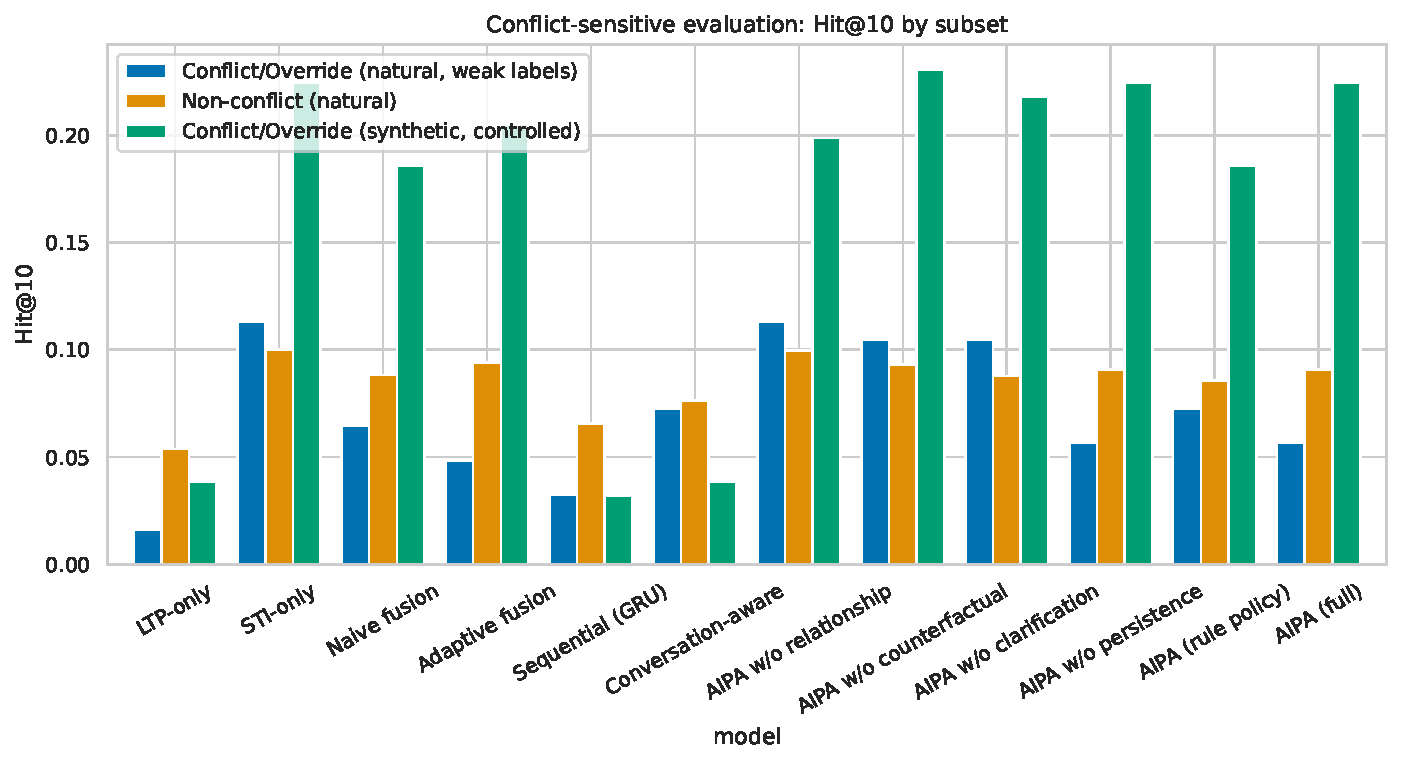
\includegraphics[width=\columnwidth]{fig04_conflict_vs_nonconflict}
  \caption{Hit@10 on natural conflict versus non-conflict turns. Intervals on the conflict side are wide because the subset is small.}
  \label{fig:conflict}
\end{figure}

Figure~\ref{fig:subsets} breaks the natural set down by all five relationship classes. The \emph{Uncertain} class (336 instances, a third of them cold seekers) is where the intent-only model gains most of its edge; \emph{Consistent} turns, the majority, show all fused models within a few thousandths of each other.

\begin{figure}[t]
  \centering
  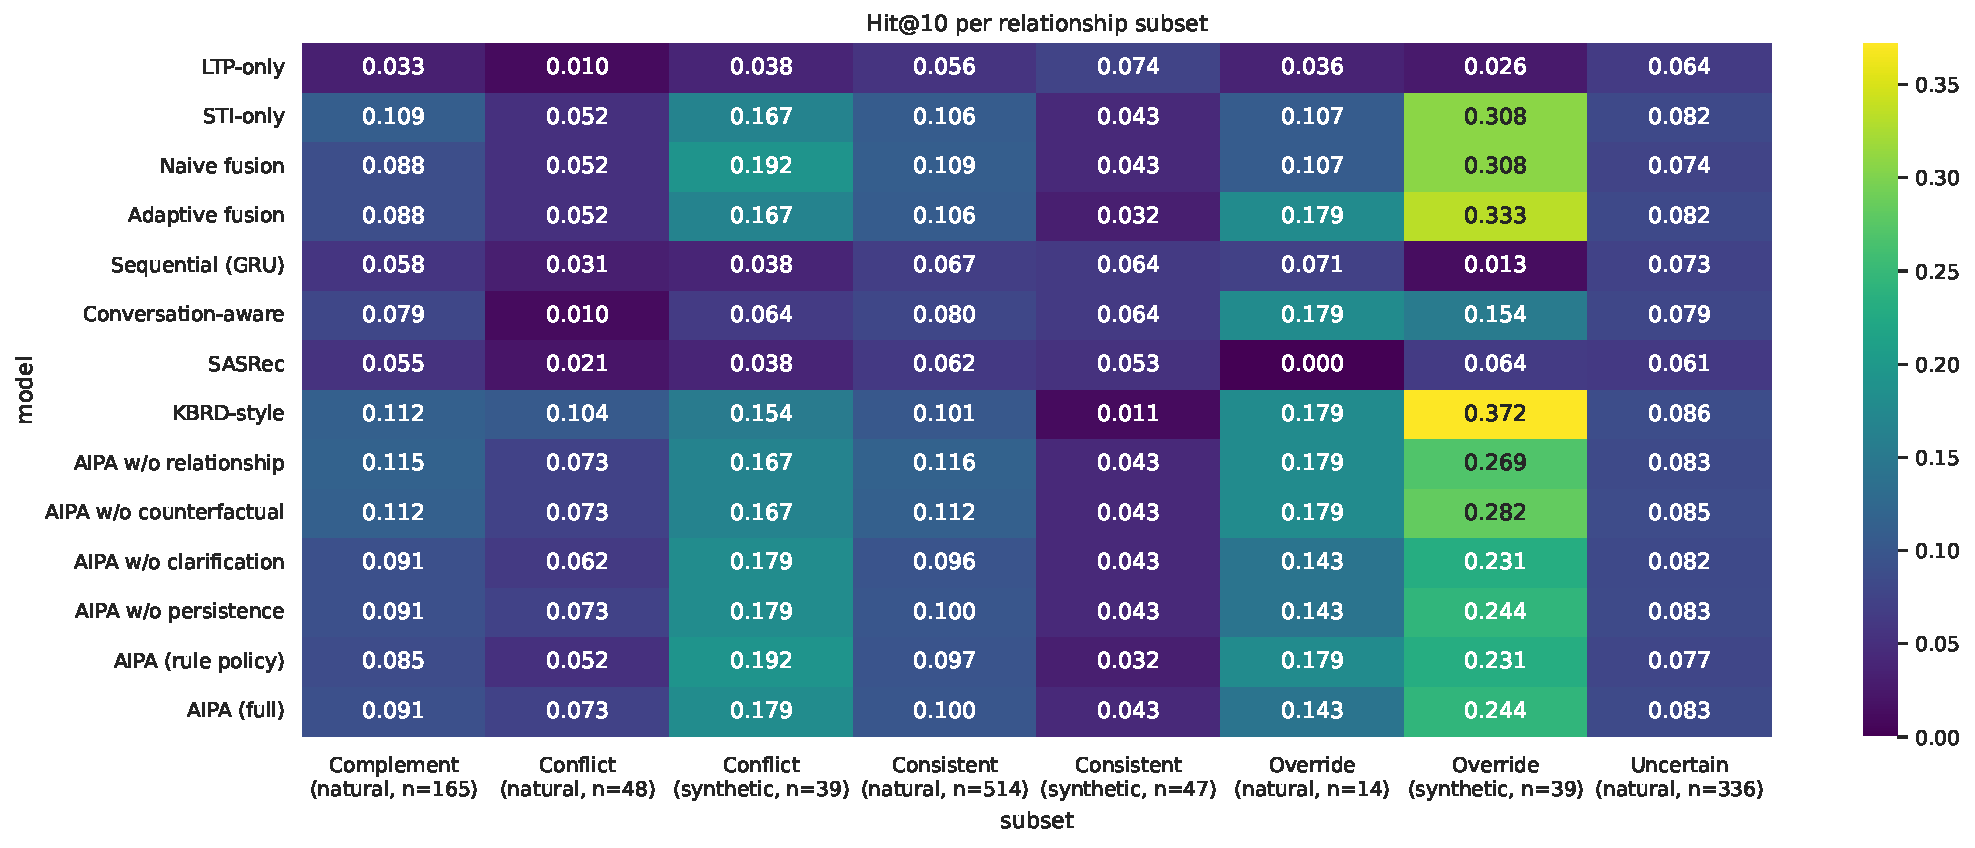
\includegraphics[width=\columnwidth]{fig05_relationship_subsets}
  \caption{Hit@10 per relationship class on natural (weak-rule) and synthetic labels.}
  \label{fig:subsets}
\end{figure}

\subsection{Relationship classification and arbitration}
Table~\ref{tab:rel} reports the relationship head. On natural data accuracy is 0.73--0.76 and macro-F1 0.52--0.55; the head is good at \emph{Consistent} and \emph{Uncertain} (F1 0.79--0.94), mediocre at \emph{Override} (about 0.4) and poor at \emph{Conflict} (about 0.2). Two caveats: the reference labels are themselves weak, so part of this ``error'' is label noise, and \emph{Conflict} has only 48 natural test instances. On synthetic data the head is near-perfect on \emph{Conflict} and \emph{Override} (F1 above 0.93), which shows it can recognise the pattern when the text states it plainly; the \emph{Complement} and \emph{Uncertain} columns are empty there because those classes are never injected. The confusion matrix in Fig.~\ref{fig:confusion} shows that natural conflicts are mostly absorbed into \emph{Consistent}.

\begin{table*}[t]
  \centering
  \caption{Relationship classification, mean over seeds. W-F1 is weighted F1; the last five columns are per-class F1 (--: class absent from the subset).}
  \label{tab:rel}
  \small
  \begin{tabular}{llcccccccc}
\toprule
Model & Subset & Acc. & Macro-F1 & W-F1 & Compl. & Consist. & Confl. & Overr. & Uncert. \\
\midrule
AIPA w/o relationship & natural & 0.794 & 0.621 & 0.791 & 0.521 & 0.845 & 0.422 & 0.363 & 0.953 \\
AIPA w/o relationship & synthetic & 0.971 & 0.970 & 0.970 & 0.941 & 0.970 & 0.943 & 0.996 & 1.000 \\
AIPA w/o counterfactual & natural & 0.795 & 0.621 & 0.792 & 0.534 & 0.847 & 0.406 & 0.368 & 0.951 \\
AIPA w/o counterfactual & synthetic & 0.973 & 0.973 & 0.973 & 0.947 & 0.970 & 0.951 & 0.997 & 1.000 \\
AIPA w/o clarification & natural & 0.801 & 0.617 & 0.796 & 0.549 & 0.847 & 0.400 & 0.334 & 0.956 \\
AIPA w/o clarification & synthetic & 0.965 & 0.964 & 0.965 & 0.934 & 0.968 & 0.929 & 0.992 & 1.000 \\
AIPA w/o persistence & natural & 0.807 & 0.656 & 0.804 & 0.556 & 0.854 & 0.444 & 0.471 & 0.954 \\
AIPA w/o persistence & synthetic & 0.963 & 0.962 & 0.962 & 0.927 & 0.961 & 0.931 & 0.988 & 1.000 \\
AIPA (rule policy) & natural & 0.802 & 0.636 & 0.799 & 0.543 & 0.852 & 0.427 & 0.406 & 0.953 \\
AIPA (rule policy) & synthetic & 0.967 & 0.966 & 0.967 & 0.936 & 0.968 & 0.930 & 0.996 & 1.000 \\
AIPA (full) & natural & 0.800 & 0.627 & 0.797 & 0.553 & 0.848 & 0.412 & 0.369 & 0.954 \\
AIPA (full) & synthetic & 0.963 & 0.962 & 0.962 & 0.927 & 0.961 & 0.931 & 0.988 & 1.000 \\
\bottomrule
\end{tabular}

\end{table*}

\begin{figure}[t]
  \centering
  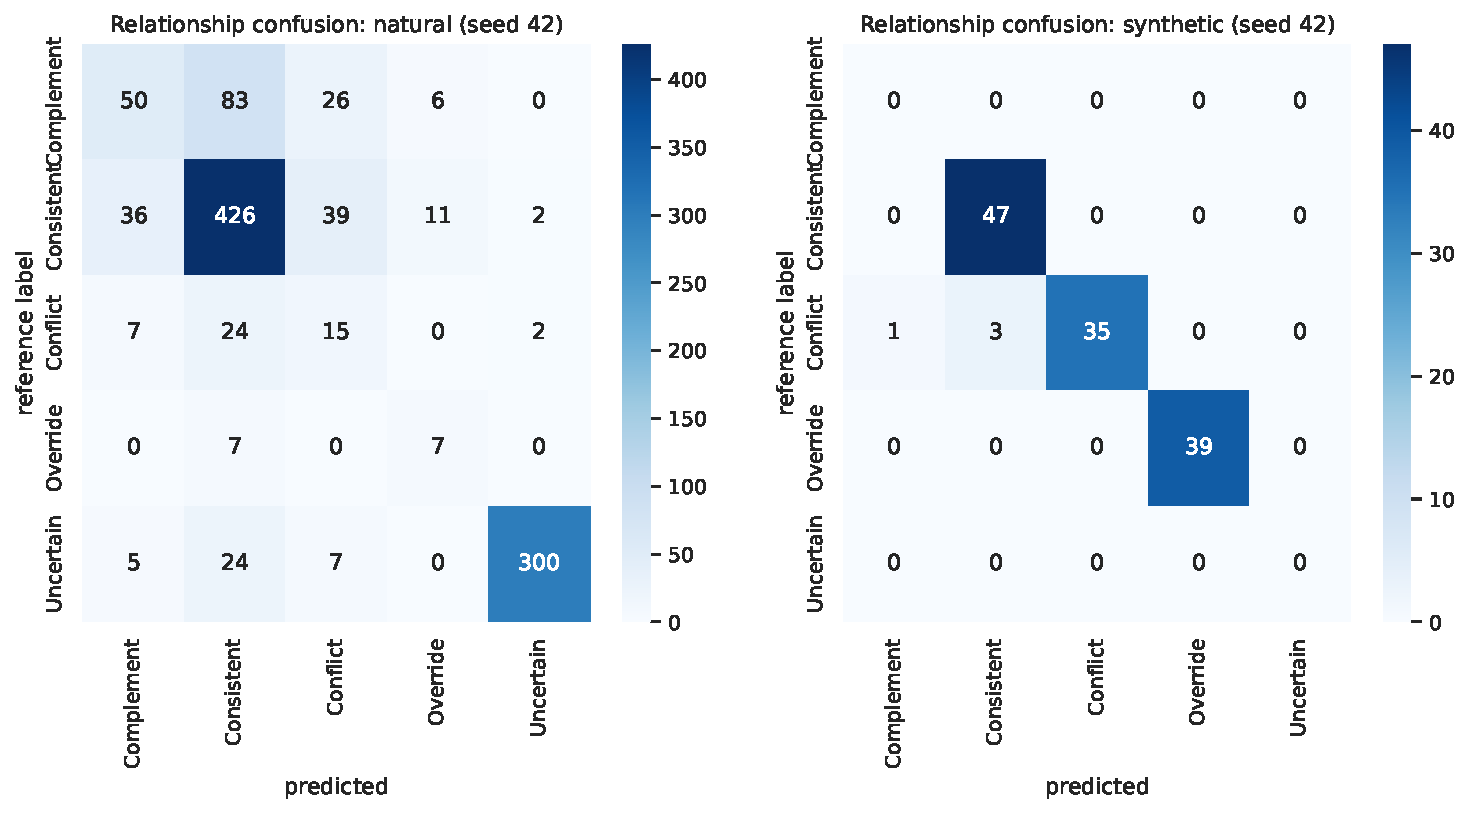
\includegraphics[width=\columnwidth]{fig06_relationship_confusion}
  \caption{Relationship confusion matrix of AIPA (full) on natural test turns (rows: weak-rule reference; columns: prediction).}
  \label{fig:confusion}
\end{figure}

The arbitration head (Table~\ref{tab:arb}, Fig.~\ref{fig:actions}) is the most encouraging part of the results. The learned policy asks a clarifying question on about 20\% of natural turns, and when it asks, the reference label is \emph{Uncertain} or \emph{Conflict} 98--99\% of the time; unnecessary clarifications are below 0.5\% and wrong overrides below 3.5\%. The rule policy asks more often (27--30\%) with markedly lower precision (0.69--0.75), so the learned policy is doing more than reproducing the table it was seeded with. Conflict-resolution accuracy on natural conflicts is low (0.15--0.26) for the reasons above; on synthetic conflicts it is 0.88--0.91. Calibration of the relationship head is acceptable (ECE 0.04--0.06 on natural data, Fig.~\ref{fig:calib}).

\begin{table*}[t]
  \centering
  \caption{Arbitration and clarification behaviour, mean over seeds. Clarification precision is undefined when no question is asked.}
  \label{tab:arb}
  \small
  \begin{tabular}{llccccccc}
\toprule
Model & Subset & Arb.\ acc. & Confl.\ res. & Overr.\ succ. & Clar.\ rate & Clar.\ prec. & Unnec.\ clar. & Wrong overr. \\
\midrule
AIPA w/o relationship & natural & 0.894 & 0.418 & 0.200 & 0.196 & 0.989 & 0.002 & 0.017 \\
AIPA w/o relationship & synthetic & 0.980 & 0.958 & 0.205 & 0.226 & 1.000 & 0.000 & 0.000 \\
AIPA w/o counterfactual & natural & 0.892 & 0.414 & 0.218 & 0.199 & 0.979 & 0.004 & 0.014 \\
AIPA w/o counterfactual & synthetic & 0.984 & 0.963 & 0.209 & 0.226 & 1.000 & 0.000 & 0.000 \\
AIPA w/o clarification & natural & 0.709 & 0.351 & 0.306 & 0.000 & -- & 0.000 & 0.010 \\
AIPA w/o clarification & synthetic & 0.750 & 0.937 & 0.203 & 0.000 & -- & 0.000 & 0.000 \\
AIPA w/o persistence & natural & 0.905 & 0.406 & 0.196 & 0.196 & 0.991 & 0.002 & 0.011 \\
AIPA w/o persistence & synthetic & 0.974 & 0.938 & 0.208 & 0.226 & 1.000 & 0.000 & 0.000 \\
AIPA (rule policy) & natural & 0.811 & 0.286 & 0.393 & 0.323 & 0.642 & 0.116 & 0.009 \\
AIPA (rule policy) & synthetic & 0.952 & 0.900 & 0.214 & 0.257 & 0.880 & 0.031 & 0.000 \\
AIPA (full) & natural & 0.902 & 0.353 & 0.263 & 0.196 & 0.991 & 0.002 & 0.010 \\
AIPA (full) & synthetic & 0.974 & 0.938 & 0.208 & 0.226 & 1.000 & 0.000 & 0.000 \\
\bottomrule
\end{tabular}

\end{table*}

\begin{figure}[t]
  \centering
  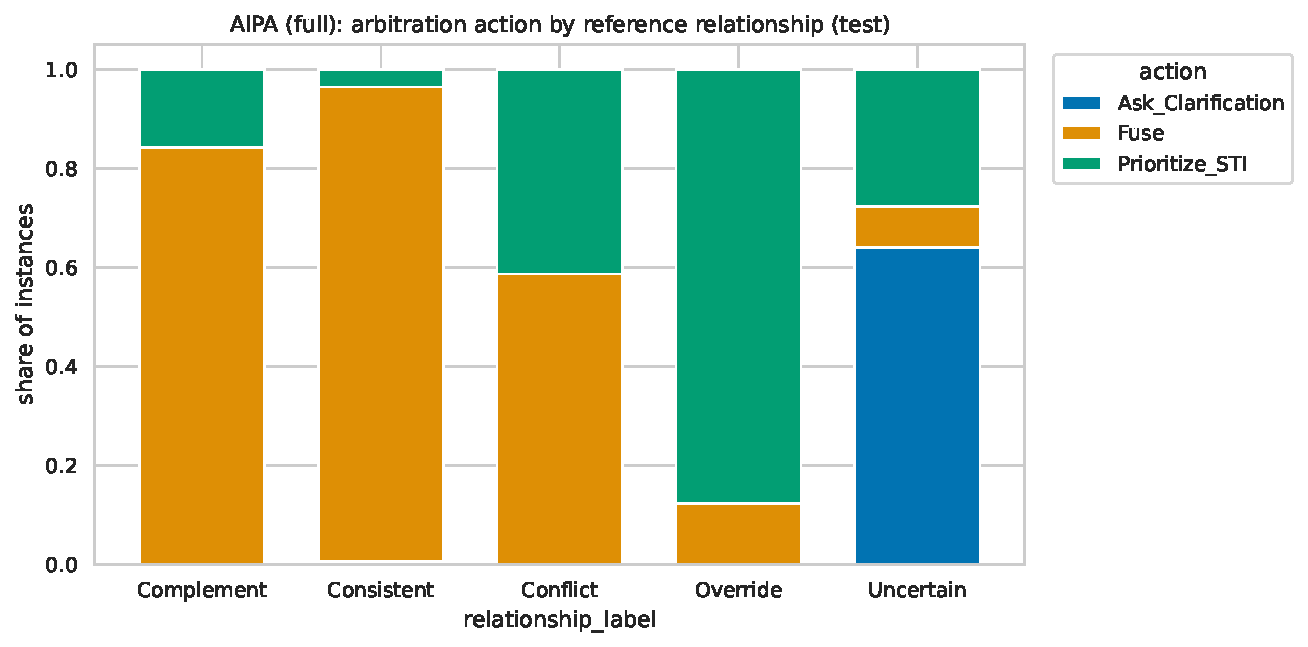
\includegraphics[width=\columnwidth]{fig07_actions_by_relationship}
  \caption{Distribution of predicted actions within each reference relationship class, AIPA (full), natural turns.}
  \label{fig:actions}
\end{figure}

\begin{figure}[t]
  \centering
  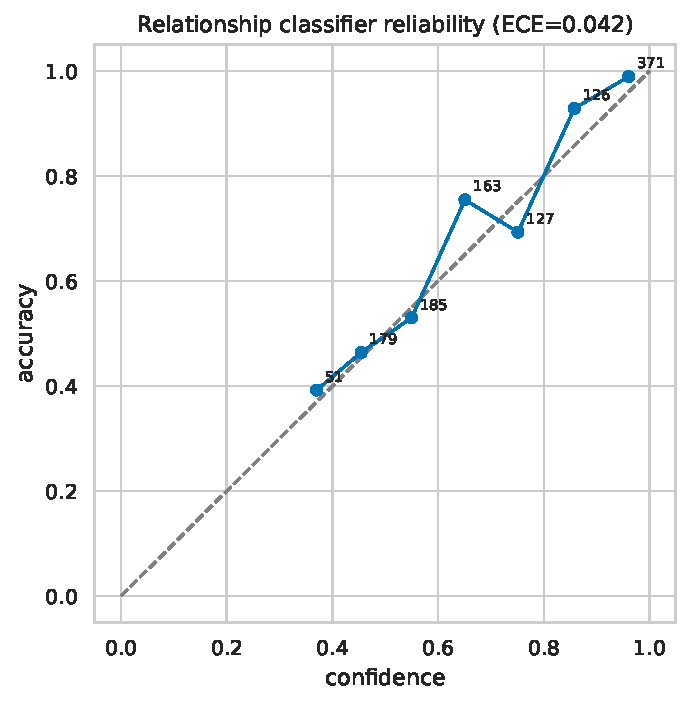
\includegraphics[width=\columnwidth]{fig11_calibration}
  \caption{Reliability diagram of the relationship head.}
  \label{fig:calib}
\end{figure}

\subsection{Counterfactual driver diagnostic}
Table~\ref{tab:cf} and Fig.~\ref{fig:cf} summarise the intervention probe for AIPA (full). Removing the STI pathway disrupts the top-10 list far more than removing LTP (overlap with the original list about 0.15--0.24 versus 0.62--0.74 on natural turns), and the per-turn driver label is \emph{STI-driven} or \emph{Jointly-driven} almost everywhere; \emph{LTP-driven} turns are essentially absent and no turn is \emph{Neither-driven}. On synthetic conflicts and overrides the STI dependence is strongest (overlap without STI 0.06), which is what one would want. Agreement between the driver label and the chosen action is 0.46 on natural turns and 0.62 on synthetic turns. The diagnostic thus confirms what the ranking tables already suggest: the trained model leans heavily on the conversation and uses the profile as a secondary signal.

\begin{table*}[t]
  \centering
  \caption{Counterfactual probe of AIPA (full) by relationship class: mean absolute change in NDCG@10 and top-10 overlap when one pathway is removed, and the share of turns assigned to each driver label. These describe the model, not the users.}
  \label{tab:cf}
  \small
  \begin{tabular}{llr cc cc cccc}
\toprule
& & & \multicolumn{2}{c}{$|\Delta$NDCG@10$|$} & \multicolumn{2}{c}{Top-10 overlap} & \multicolumn{4}{c}{Driver (\%)} \\
\cmidrule(lr){4-5}\cmidrule(lr){6-7}\cmidrule(lr){8-11}
Source & Relationship & $n$ & no LTP & no STI & no LTP & no STI & STI & LTP & Joint & Neither \\
\midrule
natural & Complement & 165 & 0.027 & 0.056 & 0.613 & 0.210 & 40 & 1 & 59 & 0 \\
natural & Conflict & 48 & 0.024 & 0.033 & 0.567 & 0.191 & 35 & 1 & 64 & 0 \\
natural & Consistent & 514 & 0.027 & 0.048 & 0.609 & 0.280 & 43 & 1 & 55 & 0 \\
natural & Override & 14 & 0.043 & 0.074 & 0.725 & 0.168 & 54 & 0 & 46 & 0 \\
natural & Uncertain & 336 & 0.014 & 0.050 & 0.718 & 0.305 & 57 & 1 & 42 & 0 \\
synthetic & Complement & 31 & 0.089 & 0.091 & 0.621 & 0.200 & 42 & 0 & 58 & 0 \\
synthetic & Conflict & 33 & 0.021 & 0.127 & 0.848 & 0.020 & 82 & 0 & 18 & 0 \\
synthetic & Consistent & 24 & 0.020 & 0.027 & 0.579 & 0.315 & 35 & 0 & 65 & 0 \\
synthetic & Override & 24 & 0.039 & 0.122 & 0.875 & 0.017 & 85 & 0 & 15 & 0 \\
synthetic & Uncertain & 31 & 0.028 & 0.070 & 0.569 & 0.487 & 27 & 2 & 71 & 0 \\
\bottomrule
\end{tabular}

\end{table*}

\begin{figure}[t]
  \centering
  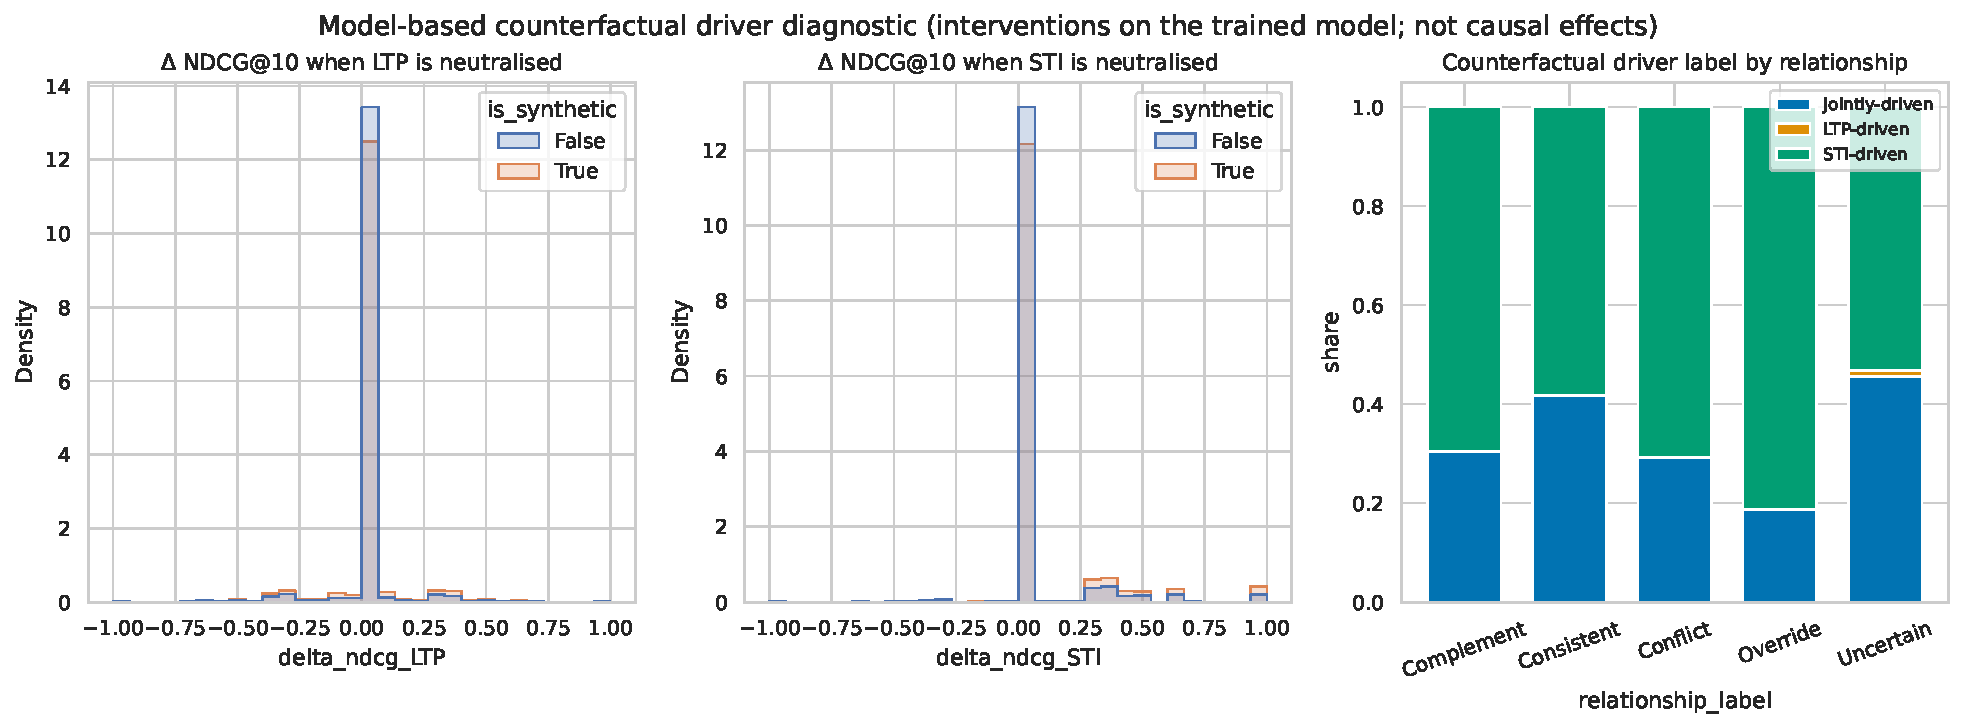
\includegraphics[width=\columnwidth]{fig08_counterfactual}
  \caption{Driver-label distribution and NDCG changes under signal removal.}
  \label{fig:cf}
\end{figure}

\subsection{Persistent shifts}
The tracker flagged 33 persistent shifts across all AIPA variants and seeds (e.g.\ seeker 1087 repeatedly steering toward war films, seeker 1008 toward horror). Because these shifts are only applied to instances that come \emph{after} the second qualifying session, and few seekers reach that point inside the sampled test set, the full model and the ``without persistence'' ablation made identical test predictions. The mechanism works as designed but is not exercised enough by this data budget to be evaluated.

\subsection{Sensitivity and fusion weight}
Figure~\ref{fig:sens} plots Hit@10 against history length, number of seeker turns and injected conflict intensity. Performance is flat to slightly decreasing with longer histories (0.114 for 0--2 history items down to 0.085 for 26--50), a hint that long profiles add noise more than signal in the current encoder. On synthetic conflicts, AIPA (full) drops from 0.31 at the mildest intensity to 0.17 at the strongest; the ablations without counterfactual features or clarification are flatter across intensities. Table~\ref{tab:alpha} shows the fixed-weight sweep for naive fusion: anything between $\alpha_{\text{LTP}}=0.25$ and $0.5$ is close to the best, and pure LTP weighting collapses to 0.022, which sets the scale for how much the profile alone can achieve here.

\begin{figure}[t]
  \centering
  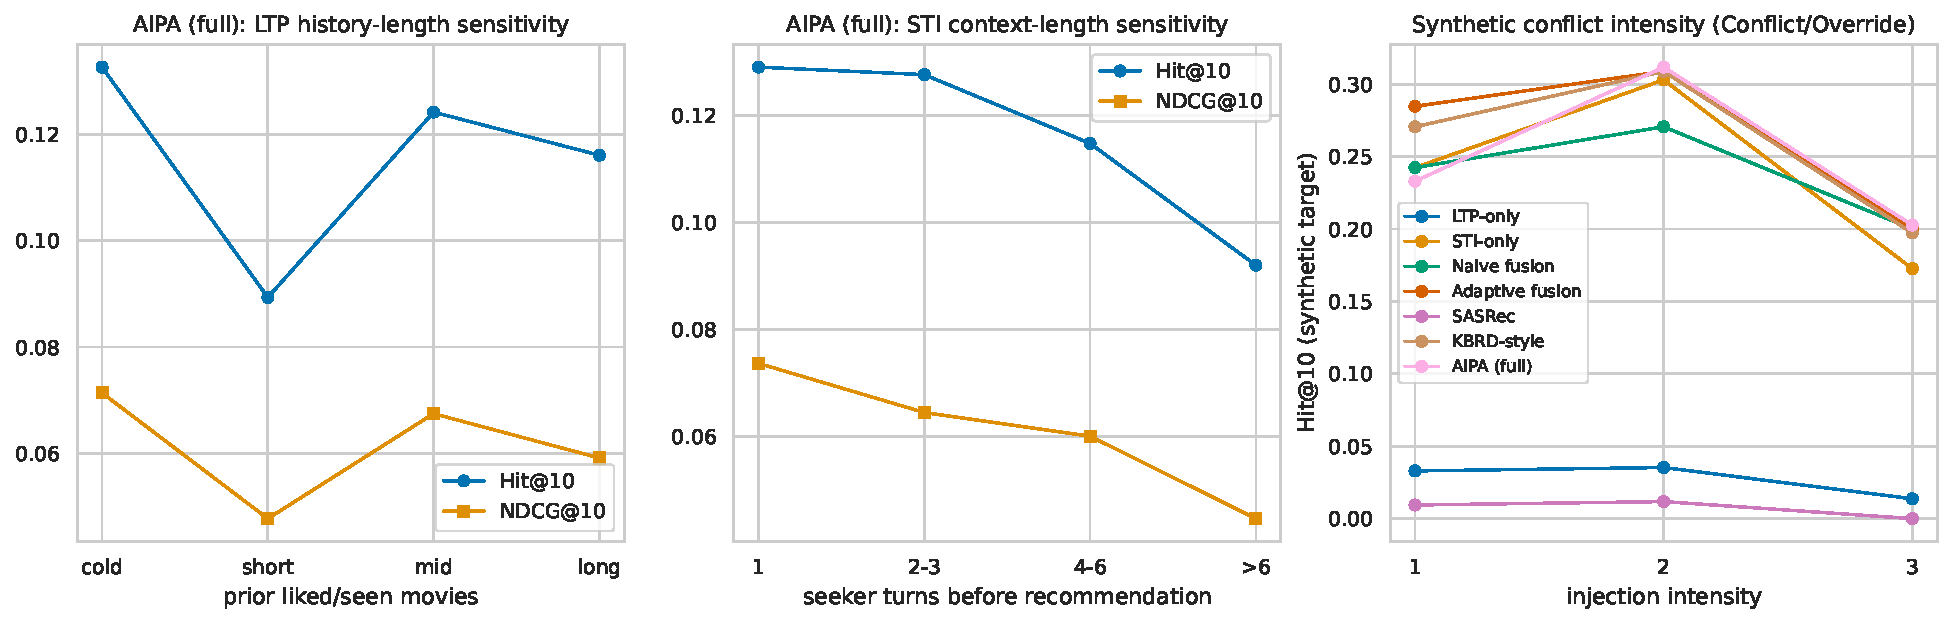
\includegraphics[width=\columnwidth]{fig09_sensitivity}
  \caption{Sensitivity of Hit@10 to history length, STI length and synthetic conflict intensity.}
  \label{fig:sens}
\end{figure}

\begin{table}[t]
  \centering
  \caption{Fixed fusion weight sweep (naive fusion, natural test set unless stated).}
  \label{tab:alpha}
  \small
  \begin{tabular}{ccccc}
\toprule
$\alpha_{\text{LTP}}$ & Hit@10 & NDCG@10 & Hit@20 & Hit@10 (synthetic) \\
\midrule
0.00 & 0.081 & 0.045 & 0.125 & 0.120 \\
0.25 & 0.088 & 0.047 & 0.133 & 0.132 \\
0.50 & 0.087 & 0.048 & 0.132 & 0.132 \\
0.75 & 0.077 & 0.041 & 0.112 & 0.112 \\
1.00 & 0.022 & 0.012 & 0.049 & 0.012 \\
\bottomrule
\end{tabular}

\end{table}

\subsection{Ablations and efficiency}
Reading the AIPA rows of Tables~\ref{tab:overall} and \ref{tab:sig} as an ablation study, none of the removals changes Hit@10 by more than 0.012 and none is significant. Removing the relationship head yields the numerically best natural score (0.100), i.e.\ the auxiliary supervision from weak labels slightly hurts ranking in this budget. All variants have 0.48--0.55\,M parameters, train in a few seconds per epoch on CPU and score a turn in under 0.05\,ms (Table~\ref{tab:eff}); the arbitration machinery costs roughly 6\% extra parameters and a factor of two in inference time relative to naive fusion, both negligible in absolute terms.

\begin{table}[t]
  \centering
  \caption{Model size and cost (CPU only).}
  \label{tab:eff}
  \scriptsize
  \resizebox{\columnwidth}{!}{\begin{tabular}{lrrrr}
\toprule
Model & Parameters & Size (MB) & Train (s) & CPU inf.\ (ms/sample) \\
\midrule
LTP-only & 597,525 & 2.39 & 19.0 & 0.032 \\
STI-only & 597,525 & 2.39 & 24.1 & 0.045 \\
Naive fusion & 597,525 & 2.39 & 21.0 & 0.093 \\
Adaptive fusion & 608,790 & 2.44 & 24.7 & 0.056 \\
Sequential (GRU) & 513,357 & 2.05 & 49.6 & 0.052 \\
Conversation-aware & 537,613 & 2.15 & 12.1 & 0.010 \\
SASRec & 546,893 & 2.19 & 355.8 & 0.067 \\
KBRD-style & 539,254 & 2.16 & 14.1 & 0.013 \\
AIPA w/o relationship & 629,150 & 2.52 & 37.3 & 0.048 \\
AIPA w/o counterfactual & 629,150 & 2.52 & 35.3 & 0.041 \\
AIPA w/o clarification & 629,470 & 2.52 & 38.5 & 0.043 \\
AIPA w/o persistence & 629,470 & 2.52 & 42.6 & 0.054 \\
AIPA (rule policy) & 617,306 & 2.47 & 42.0 & 0.062 \\
AIPA (full) & 629,470 & 2.52 & 53.1 & 0.071 \\
\bottomrule
\end{tabular}
}
\end{table}

\subsection{Qualitative cases and error analysis}
Table~\ref{tab:cases} shows representative test turns. The pattern is consistent with the aggregate numbers: when a seeker states a genre plainly (``war movies this weekend similar to Dunkirk''), the model reads it as an override, prioritises STI and ranks the target reasonably; when the request is indirect (``good old fashioned monster movies for my brother''), the STI genre cue is empty, the model asks, and the target sits far down the list. The most common error type is a weak-rule \emph{Complement} or \emph{Conflict} turn predicted as \emph{Consistent} and fused; in the natural set 77\% of \emph{Complement} and 73\% of \emph{Conflict} references are mislabelled this way, and their targets have median ranks in the 300--550 range.

\begin{table*}[t]
  \centering
  \caption{Selected test turns (N: natural, S: synthetic). Reference labels are weak-rule labels; ``Rank'' is the rank of the true target under AIPA (full).}
  \label{tab:cases}
  \scriptsize
  \resizebox{\textwidth}{!}{\begin{tabular}{@{}c p{5.6cm} p{2.6cm} p{2.6cm} p{2.0cm} l c l r@{}}
\toprule
& Dialogue excerpt (seeker turns before the target) & LTP profile & STI signal & Ref./pred.\ relationship & Action & $w_{\text{LTP}}/w_{\text{STI}}$ & Driver & Rank \\
\midrule
N & Recommender: Hello | Recommender: What kind of movies are you into ?! | Seeker: Hi!  How about inspirational war movies like PT 109  (1963) or USS Indianapolis: Men of... & Horror 0.35; Drama 0.23; Thriller 0.15 & War 0.75; Action 0.12; Drama 0.12 & Complement / Conflict & Prioritize\_STI & 0.43/0.57 & STI & 7 \\ \addlinespace
N & Recommender: Good morning. Have any plans for the weekend? | Seeker: Good morning. | Seeker: Yes, to watch a bunch of animated movies! Like The Incredibles (2004) to g... & Comedy 0.24; Animation 0.22; Children 0.17 & Animation 0.61; Action 0.11; Adventure 0.11 & Consistent / Consistent & Fuse & 0.49/0.51 & Jointly & 3 \\ \addlinespace
N & Recommender: One of my favorites is The Jerk (1979). Have you seen it? | Seeker: I've never seen it | Recommender: It's a bit older. Tropic Thunder (2008) is more rece... & Drama 0.28; Action 0.19; Adventure 0.10 & Comedy 1.00 & Conflict / Consistent & Fuse & 0.48/0.52 & STI & 6 \\ \addlinespace
N & Seeker: Hows it going? | Recommender: Good. | Seeker: I like pretty much anything but horror! | Seeker: Anything recent that you have seen? & Comedy 0.18; Mystery 0.14; Crime 0.11 & Horror 1.00 & Override / Consistent & Prioritize\_STI & 0.43/0.57 & STI & 144 \\ \addlinespace
N & Seeker: i am in the mood to watch movies | Recommender: Hi What kind of movies are you into | Seeker: anything you would like to recommend? | Seeker: I am open to any ... & Comedy 0.65; Romance 0.14; Crime 0.06 & (no genre cue) & Uncertain / Uncertain & Ask\_Clarification & 0.45/0.55 & Jointly & 639 \\ \addlinespace
N & Recommender: Of course I have to mention The Bodyguard  (1992) | Recommender: Awww. I thought that one was great. | Seeker: Oh, yes!  With Whitney Houston. That's one ... & Comedy 0.44; Horror 0.17; Drama 0.12 & Action 0.17; Adventure 0.17; Children 0.17 & Complement / Complement & Fuse & 0.48/0.52 & Jointly & 6167 \\ \addlinespace
N & Recommender: Hello. How are you? | Seeker: Hey there, I'm looking for a good thriller movie. Do you know any good ones? & (none: cold seeker) & Thriller 1.00 & Uncertain / Uncertain & Prioritize\_STI & 0.41/0.59 & STI & 275 \\ \addlinespace
N & Recommender: What kind of movies do you like? | Seeker: Hello | Seeker: i open to any movie & Action 0.28; Sci-Fi 0.28; Adventure 0.21 & (no genre cue) & Uncertain / Uncertain & Ask\_Clarification & 0.45/0.55 & Jointly & 44 \\ \addlinespace
\bottomrule
\end{tabular}
}
\end{table*}

\section{Discussion}
\label{sec:discussion}
\subsection{What the evidence supports}
Three things are supported by this run. (i) Any model that reads the conversation beats a profile-only model on ReDial by a wide, significant margin; the profile alone reaches about 5\% Hit@10. (ii) The learned arbitration policy is well-behaved: it asks when it should, rarely asks when it should not, and rarely overrides in the wrong direction. (iii) On plainly stated departures from habit (the synthetic set), AIPA follows the user, and the counterfactual probe shows that the ranking really is driven by the stated intent in those cases.

\subsection{What it does not support}
The central claim, that explicit arbitration improves recommendations over simpler fusion \emph{specifically on conflict turns}, is not supported here. The natural conflict subset is too small for a decisive test and its point estimates lean the wrong way; on synthetic conflicts AIPA merely ties the trivial intent-following policy. The ablations are flat. We see three reasons, in rough order of importance.

First, the labels. Weak-rule relationship labels are the reference for the relationship head, the arbitration metrics and the conflict subset itself. If the rule mislabels many turns, we are training toward noise and evaluating on a subset that is not what we think it is. The near-perfect synthetic results versus the weak natural results point in that direction.

Second, the budget. A quarter of the corpus and two seeds give 62 natural conflict turns. With Hit@10 around 0.1 that is nowhere near enough to detect a plausible effect of a few points.

Third, the representation. TF--IDF/SVD text features capture genre words and little else. Much of what makes a request an intent (``for my brother'', ``something to fall asleep to'') is invisible to the STI encoder, and so the \emph{Uncertain} class is large and cold-start heavy.

\subsection{What a conclusive test needs}
\begin{enumerate}
  \item Run the ``full'' configuration: the whole corpus, at least five seeds and 1{,}000 bootstrap resamples, so that the conflict subset has several hundred turns.
  \item Obtain human relationship annotations for a few hundred test turns. The pipeline already accepts such a file and would report all metrics against it separately; this is the single most valuable addition.
  \item Replace the text encoder by a pre-trained sentence encoder for both seeker utterances and item descriptions.
  \item Add a stronger conversational baseline trained on the same inputs (a knowledge-grounded model in the spirit of KBRD/KGSF) so that a positive result would mean something against the state of the art.
  \item Tune $\lambda_{\text{rel}}$, $\lambda_{\text{act}}$ and the persistence threshold; the relationship supervision currently costs a little ranking quality, and the persistence tracker was never exercised.
  \item Evaluate clarification with users, or at least with simulated answers; offline precision says nothing about whether a question was welcome.
\end{enumerate}

\subsection{Threats to validity}
Conversation identifiers are assumed chronological; ReDial seekers are crowd workers, not organic users, so cross-session ``preferences'' may partly reflect task instructions; the MovieLens join misses a fraction of titles, leaving those items without genres; and the ``sequential'' and ``conversation-aware'' baselines are our own small re-implementations. All of these are documented in the released code and reported in the generated experiment report.

\section{Conclusion}
We set out to make the reconciliation of long-term preference and short-term intent explicit in a conversational recommender and to test whether doing so helps where it should, on turns where the two disagree. We built a complete, reproducible pipeline on an English corpus, with leak-free cross-session histories, two clearly separated label sources, a relationship classifier, a learned arbitration policy with clarification, a persistence tracker and a counterfactual probe, and we evaluated it with intervals and corrected paired tests. The reduced-budget results show a policy that behaves sensibly and a model that follows clearly stated intent, but they do not show a ranking advantage over simpler fusion, and we have not hidden that. The next step is not another model component but better labels and a larger run; the code is ready for both.

\balance
\bibliographystyle{IEEEtran}
\bibliography{refs}

\end{document}
